\documentclass{beamer}

\mode<presentation>
  \setbeamercovered{transparent}
%  \usecolortheme{seahorse}
  \usecolortheme{default}
%  \usecolortheme{wolverine}
%  \useoutertheme{infolines}

\usepackage{listings}
\usepackage[usenames,dvipsnames,svgnames,table]{xcolor}
\usepackage{tikz}
\usepackage{pstricks}
\usepackage[T1]{fontenc}
\usepackage[serbian]{babel}
\usepackage[cp1250]{inputenc}
\usepackage{times}

\usepackage{graphics}
\usepackage{eurosym}
\usepackage{multirow}
\usepackage{multimedia}
\usepackage{color}
\usepackage{multirow}
%\usepackage{subfig}


\title[Simulacija mre\v ze u ns-3 simulatoru \hspace{1em} {\scriptsize \insertframenumber\ / \inserttotalframenumber}]
{Simulacija dinami\v ckog rutiranja u mre\v znom simulatoru ns3\\[3ex]
\small
projekat iz predmeta\\
Principi modernih telekomunikacija (IR3PMT)\\
2015.}

\author[J. \v Zivkovi\' c --- IR3PMT 2015.]{Jelena \v Zivkovi\' c}

\date[]{}


%\AtBeginSection[]
%{
%  \begin{frame}<beamer>
%    \frametitle{Sadrzaj}
%    \tableofcontents[currentsection,hideothersubsections]
%  \end{frame}
%}


%\beamerdefaultoverlayspecification{<+->}
\begin{document}

\begin{frame}
%  \vfill
  \titlepage
\end{frame}


\begin{frame}
    \frametitle{Sadr\v zaj}
    \tableofcontents
\end{frame}


\section{Uvod (o ns-3)}
% nazivi odeljaka ce se prikazati u sadrzaju

\begin{frame}
 \frametitle{Uvod}

\midskip 
\begin{block}{ns-3 simulator}
\begin{itemize}
	\item	simulacija fiksnih i be\v zi\v cnih telekomunikacionih mre\v za
	\item	ns-2 i ns-3
	\item	Linux okru\v zenje
  \end{itemize}
  \end{block}

\end{frame}
\begin{frame}
\titlename{Organizacija simulacionog modela ns-3}
\begin{columns}[T]
   \begin{column}{.5\textwidth}
\begin{figure}[t]
		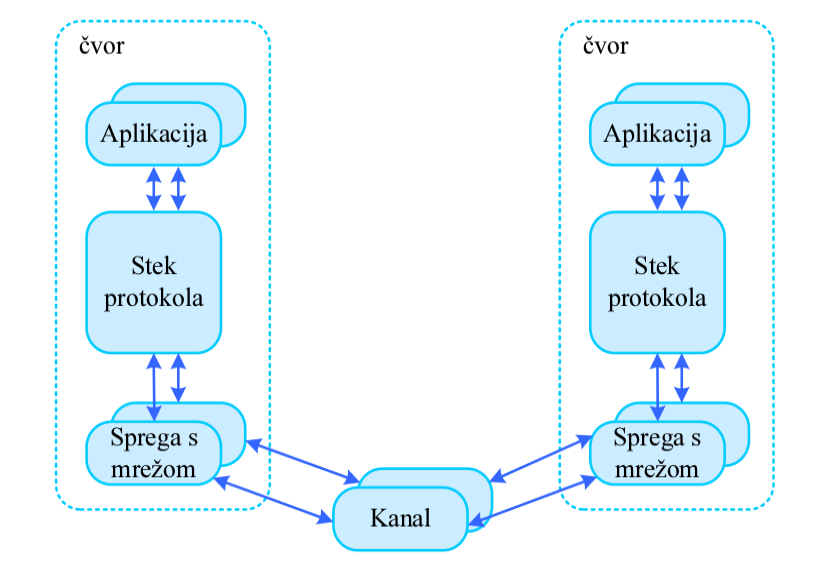
\includegraphics[width=0.6\textwidth]{slike/nov.png}
\end{figure}
 \end{column}

\begin{column}{.5\textwidth}

   \bigskip
   
   \bigskip
   
  \begin{block}{}
\begin{itemize}
   \item	Elementi mre\v ze
	\item	Aplikacije za generisanje saobra\' caja
  \end{itemize}
\end{block}{}
\end{column}
\end{columns}

\end{frame}

\begin{frame}
\frametitle{Dinami\v cko rutiranje}

\begin{columns}[T]
   \begin{column}{.5\textwidth}
\begin{figure}[t]
		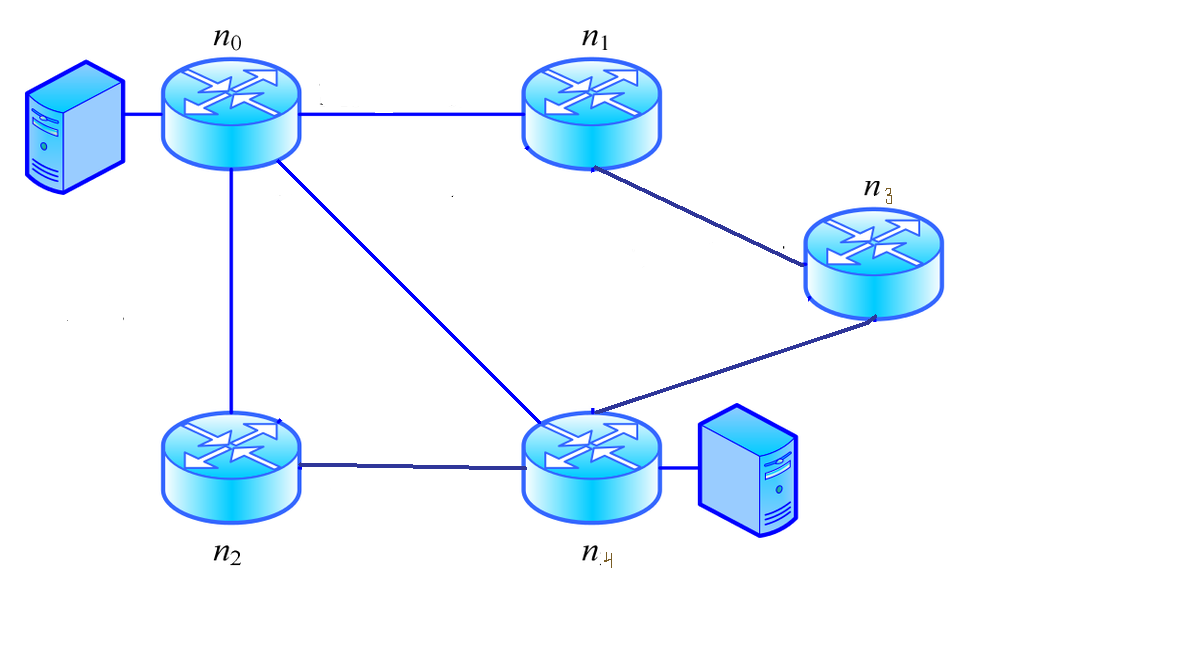
\includegraphics[width=0.6\textwidth]{slike/nov1.png}
\end{figure}
 \end{column}

\begin{column}{.5\textwidth}

   \bigskip
   
   \bigskip
   
  \begin{block}{}
\begin{itemize}

	\item u trenutku t=1s,izvor po\v cinje emitovati saobra\v caj vr\v snim protokom 100 kb/s,
uz veli\v cinu TCP paketa 150 B,
\item u trenutku t =2 s, ukida se link izmedju \v cvorova n2 i n4 ,
\item u trenutku t =3 s, ukida se link izmedju \v cvorova n0 i n4 ,
\item u trenutku t =4 s, ponovo se uspostavlja link izmedju \v cvorova n2 i n4
\item u trenutku t =5 s, isklju\v cuje se izvor.\\
  \end{itemize}
\end{block}{}
\end{column}
\end{columns}

\end{frame}


\begin{frame}
\frametitle{Parametri linkova}
\begin{figure}[t]
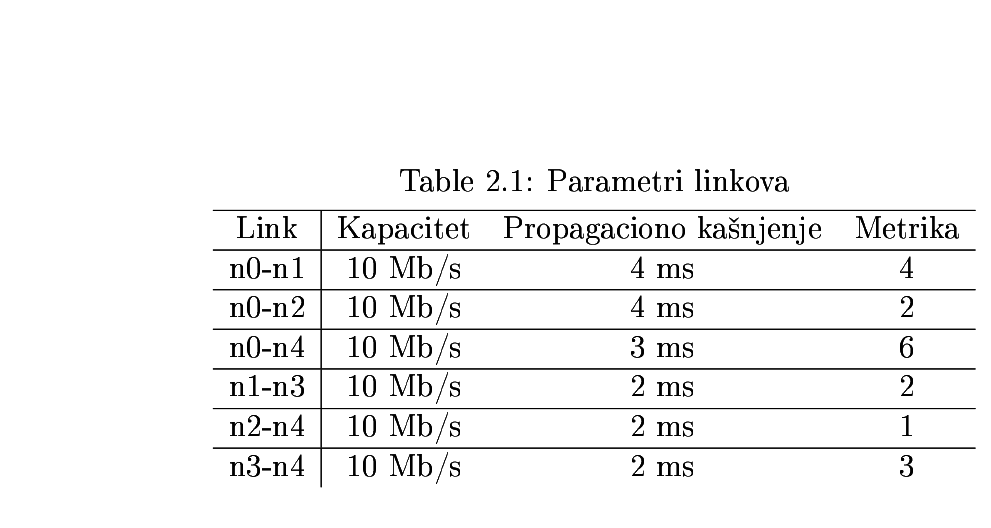
\includegraphics[width=0.9\textwidth]{slike/table.png}
\end{figure}

\end{frame}

\begin{frame}

\begin{block}{Opis simulacije} 

\begin{itemize}

	\item	\v cvoru n0 pridru\v zimo izvor saobracaja
	\item	Prijemnik paketa pridru\v zimo \v cvoru n5
	\item	Postavimo metriku uz pomo\' c metode SetMetric
	\item	metodom Simulator::Schedule specificiramo dogadjaje
	\item	Snimimo izve\v staj kao trace, pcap i xml datoteke
  \end{itemize}
  \end{block}
\end{frame}

\begin{frame}
\begin{block}{Rezultati} 

\begin{itemize}

	\item	Prikaz rezultata u tabeli rutiranja
	\item	n0 - n2 - n4 - n5   --1s
	\item	n0 - n4 - n5	    --2s
	\item	n0 - n1 - n3 - n4 - n5 --3s
	\item	n0 - n2 - n4 - n5   --4s
  \end{itemize}
  \end{block}
\end{frame}

\begin{frame}
\titlename{Animacija}
\begin{columns}[T]
   \begin{column}{.5\textwidth}
\begin{figure}[t]
		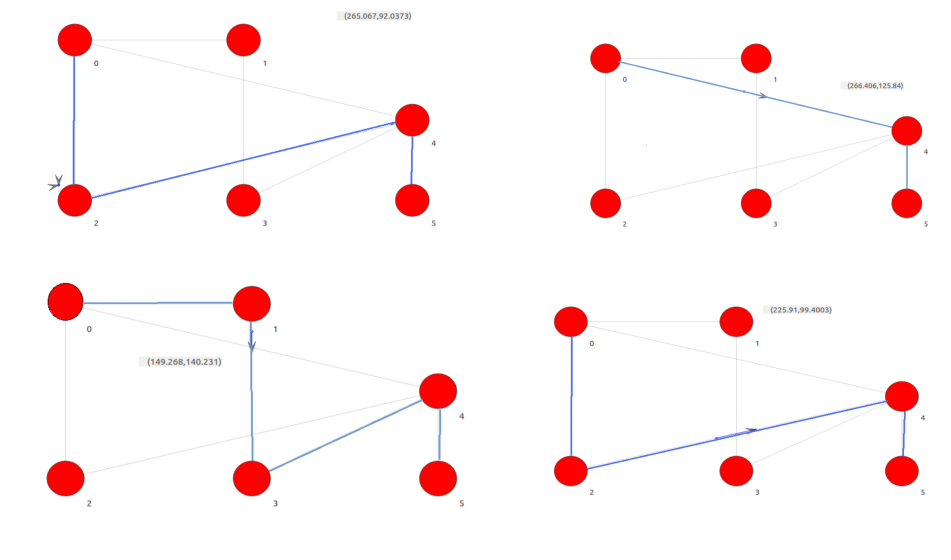
\includegraphics[width=0.6\textwidth]{slike/1.png}
\end{figure}
 \end{column}

\begin{column}{.5\textwidth}

   \bigskip
   
   \bigskip
   
  \begin{block}{}
\begin{itemize}

	\item	Stanja mre\v ze u trenucima 1s, 2s, 3s i 4s
	 \end{itemize}
\end{block}{}
\end{column}
\end{columns}
\end{frame}

\end{document}

